\documentclass[a4paper,11pt]{article}
\usepackage[utf8]{inputenc}
\usepackage{amssymb}
\usepackage{amsmath} 
\usepackage{enumerate}
\usepackage{graphicx}
\usepackage{subcaption}
\usepackage{subcaption}
\graphicspath{ {./img} }
\DeclareMathOperator*{\argmax}{arg\!\max}
\DeclareMathOperator*{\argmin}{arg\!\min}
\DeclareMathOperator*{\var}{var}
\newcounter{exercise}
\setcounter{exercise}{0}
\newcounter{subexercise}
\newcommand*{\exercise}[1][]{
  \subsection*{Exercise
    \ifx/#1/\stepcounter{exercise}\arabic{exercise}
    \else#1\fi
  }
  \setcounter{subexercise}{0}
}
\newcommand*{\subexercise}[1][]{
  \par{
    \noindent\textbf{\ifx/#1/\protect\stepcounter{subexercise}\alph{subexercise}\else#1\fi.\quad}
  }
}
\title{Chapter 24}
\author{stevenjin8}
\date{\today}

\begin{document}
  \maketitle

  \section*{Exercises}

  \begin{figure}
    \begin{subfigure}{.49\textwidth}
      \centering
      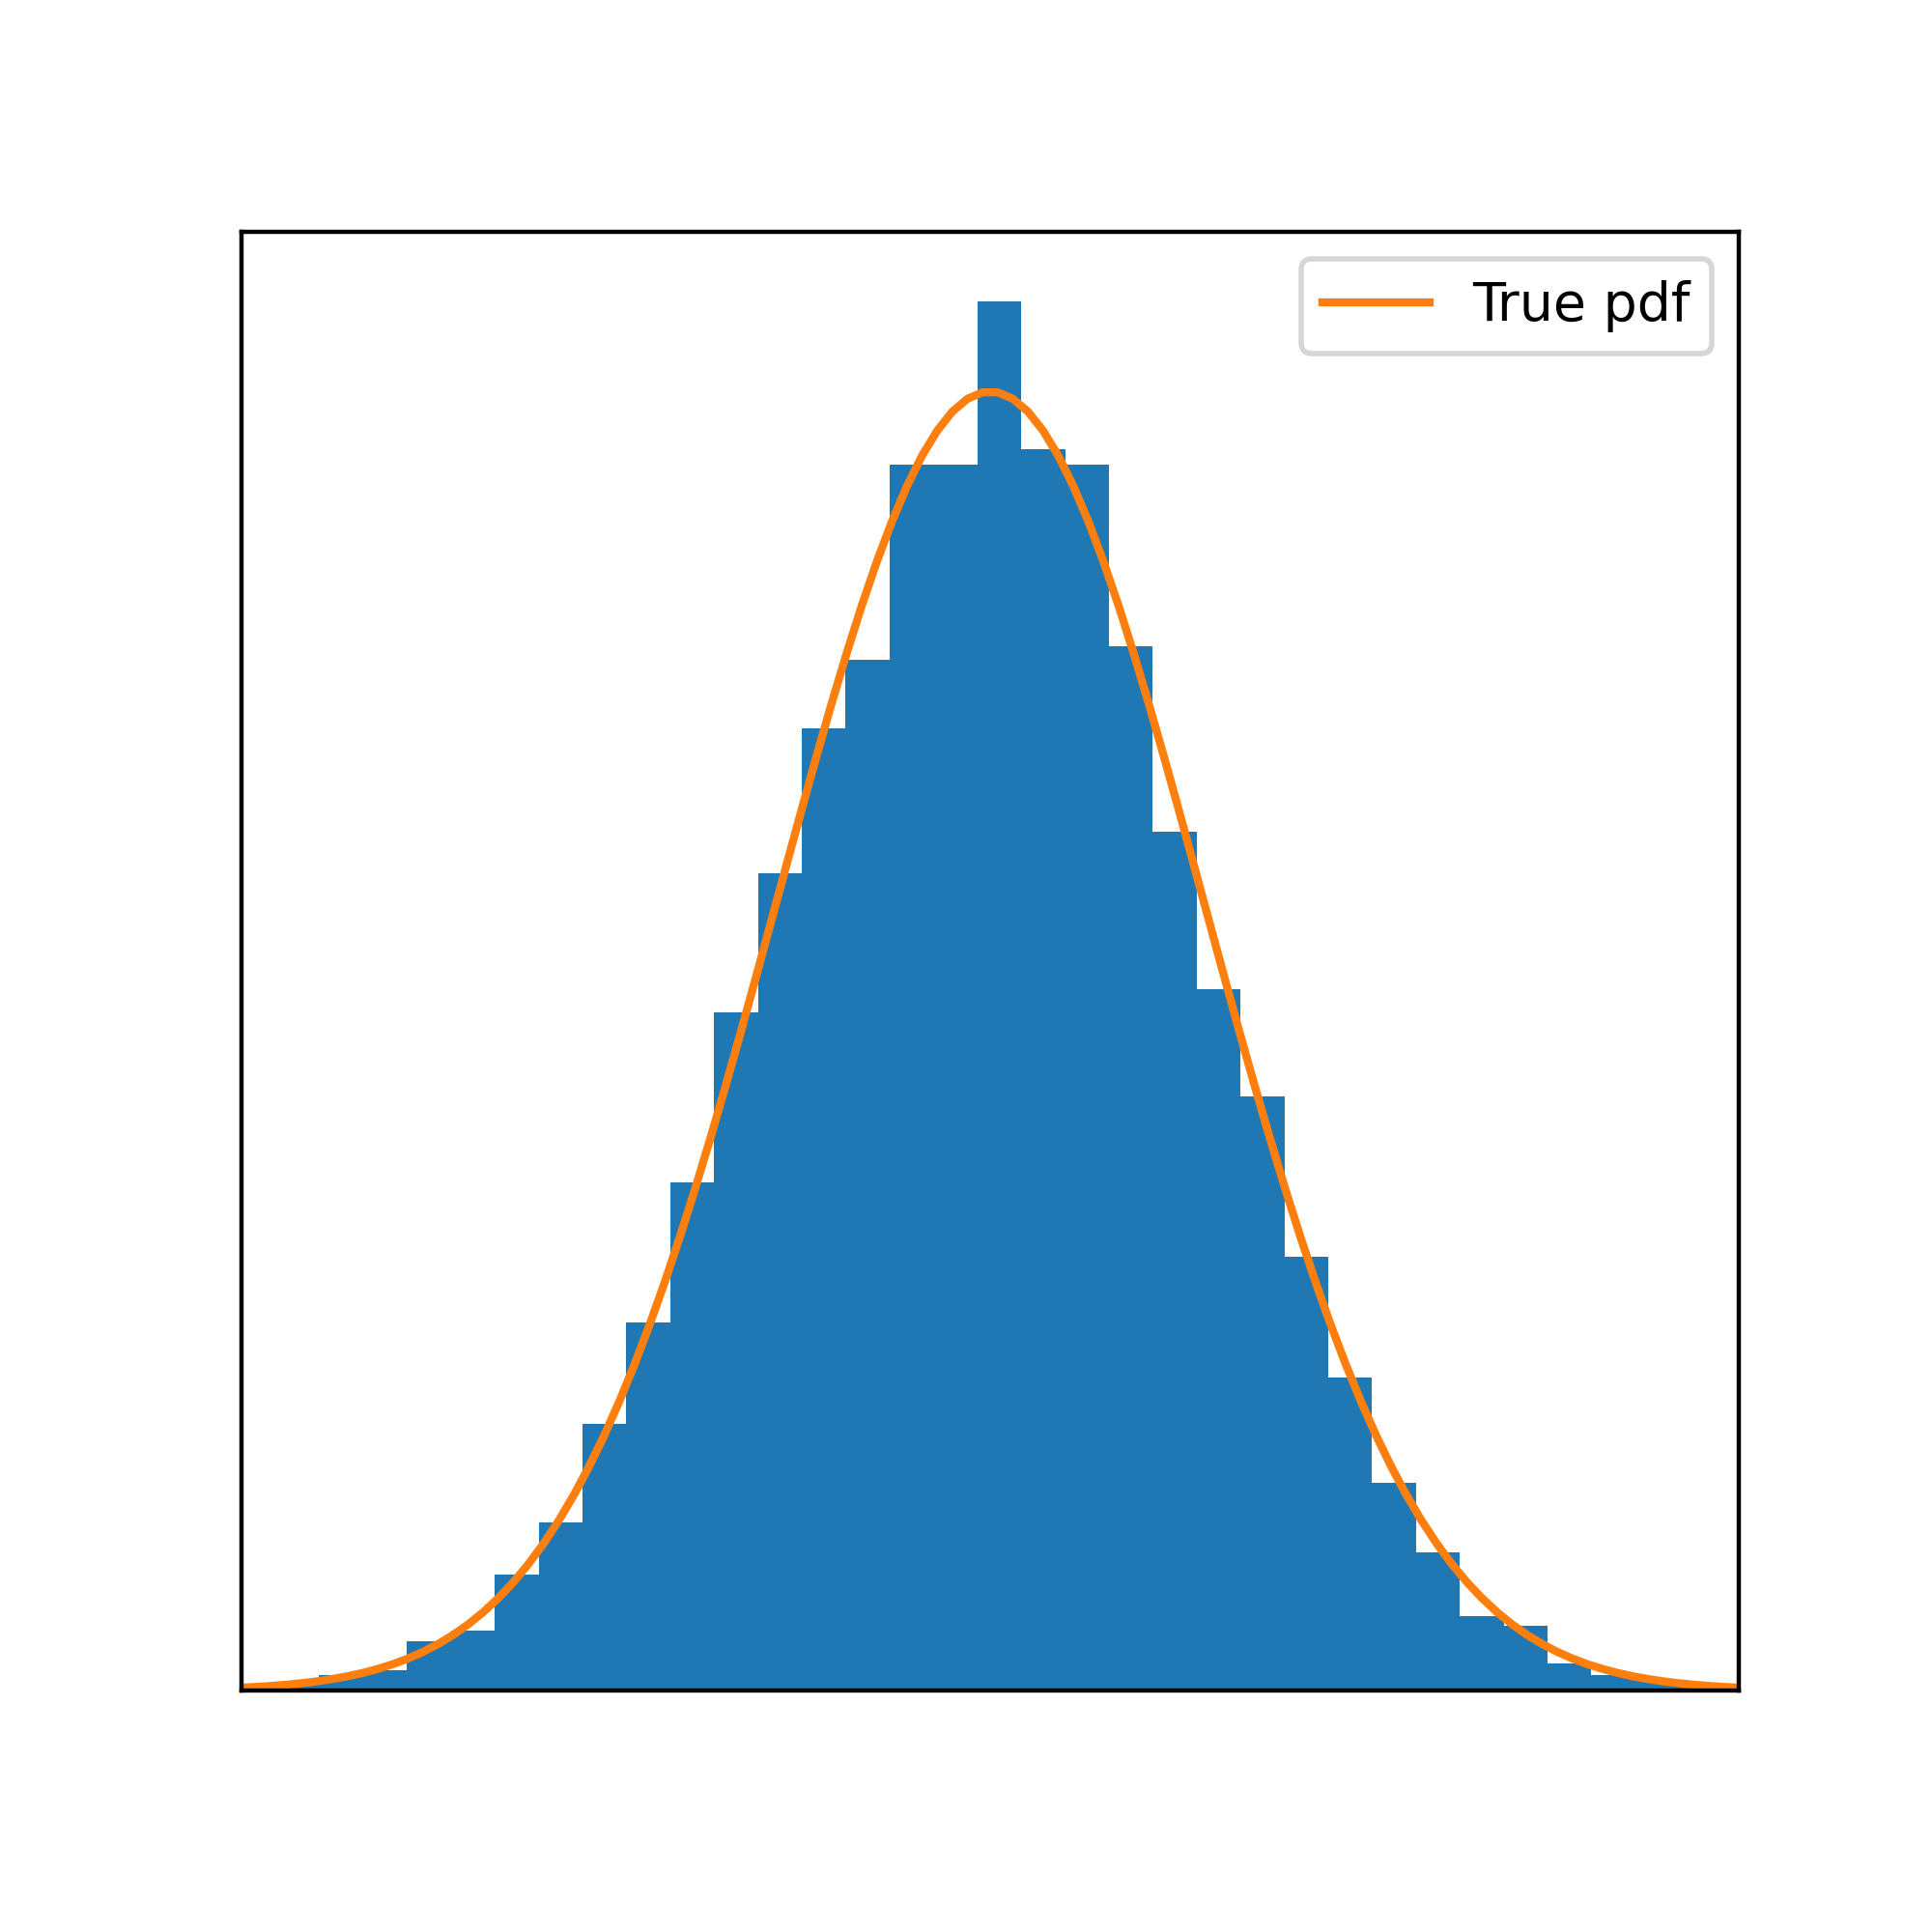
\includegraphics[width=1\linewidth]{img/gibbs/x1-hist.png}
      \caption{Empirical vs true marginal for $x_1$.}
    \end{subfigure}
    \begin{subfigure}{.49\textwidth}
      \centering
      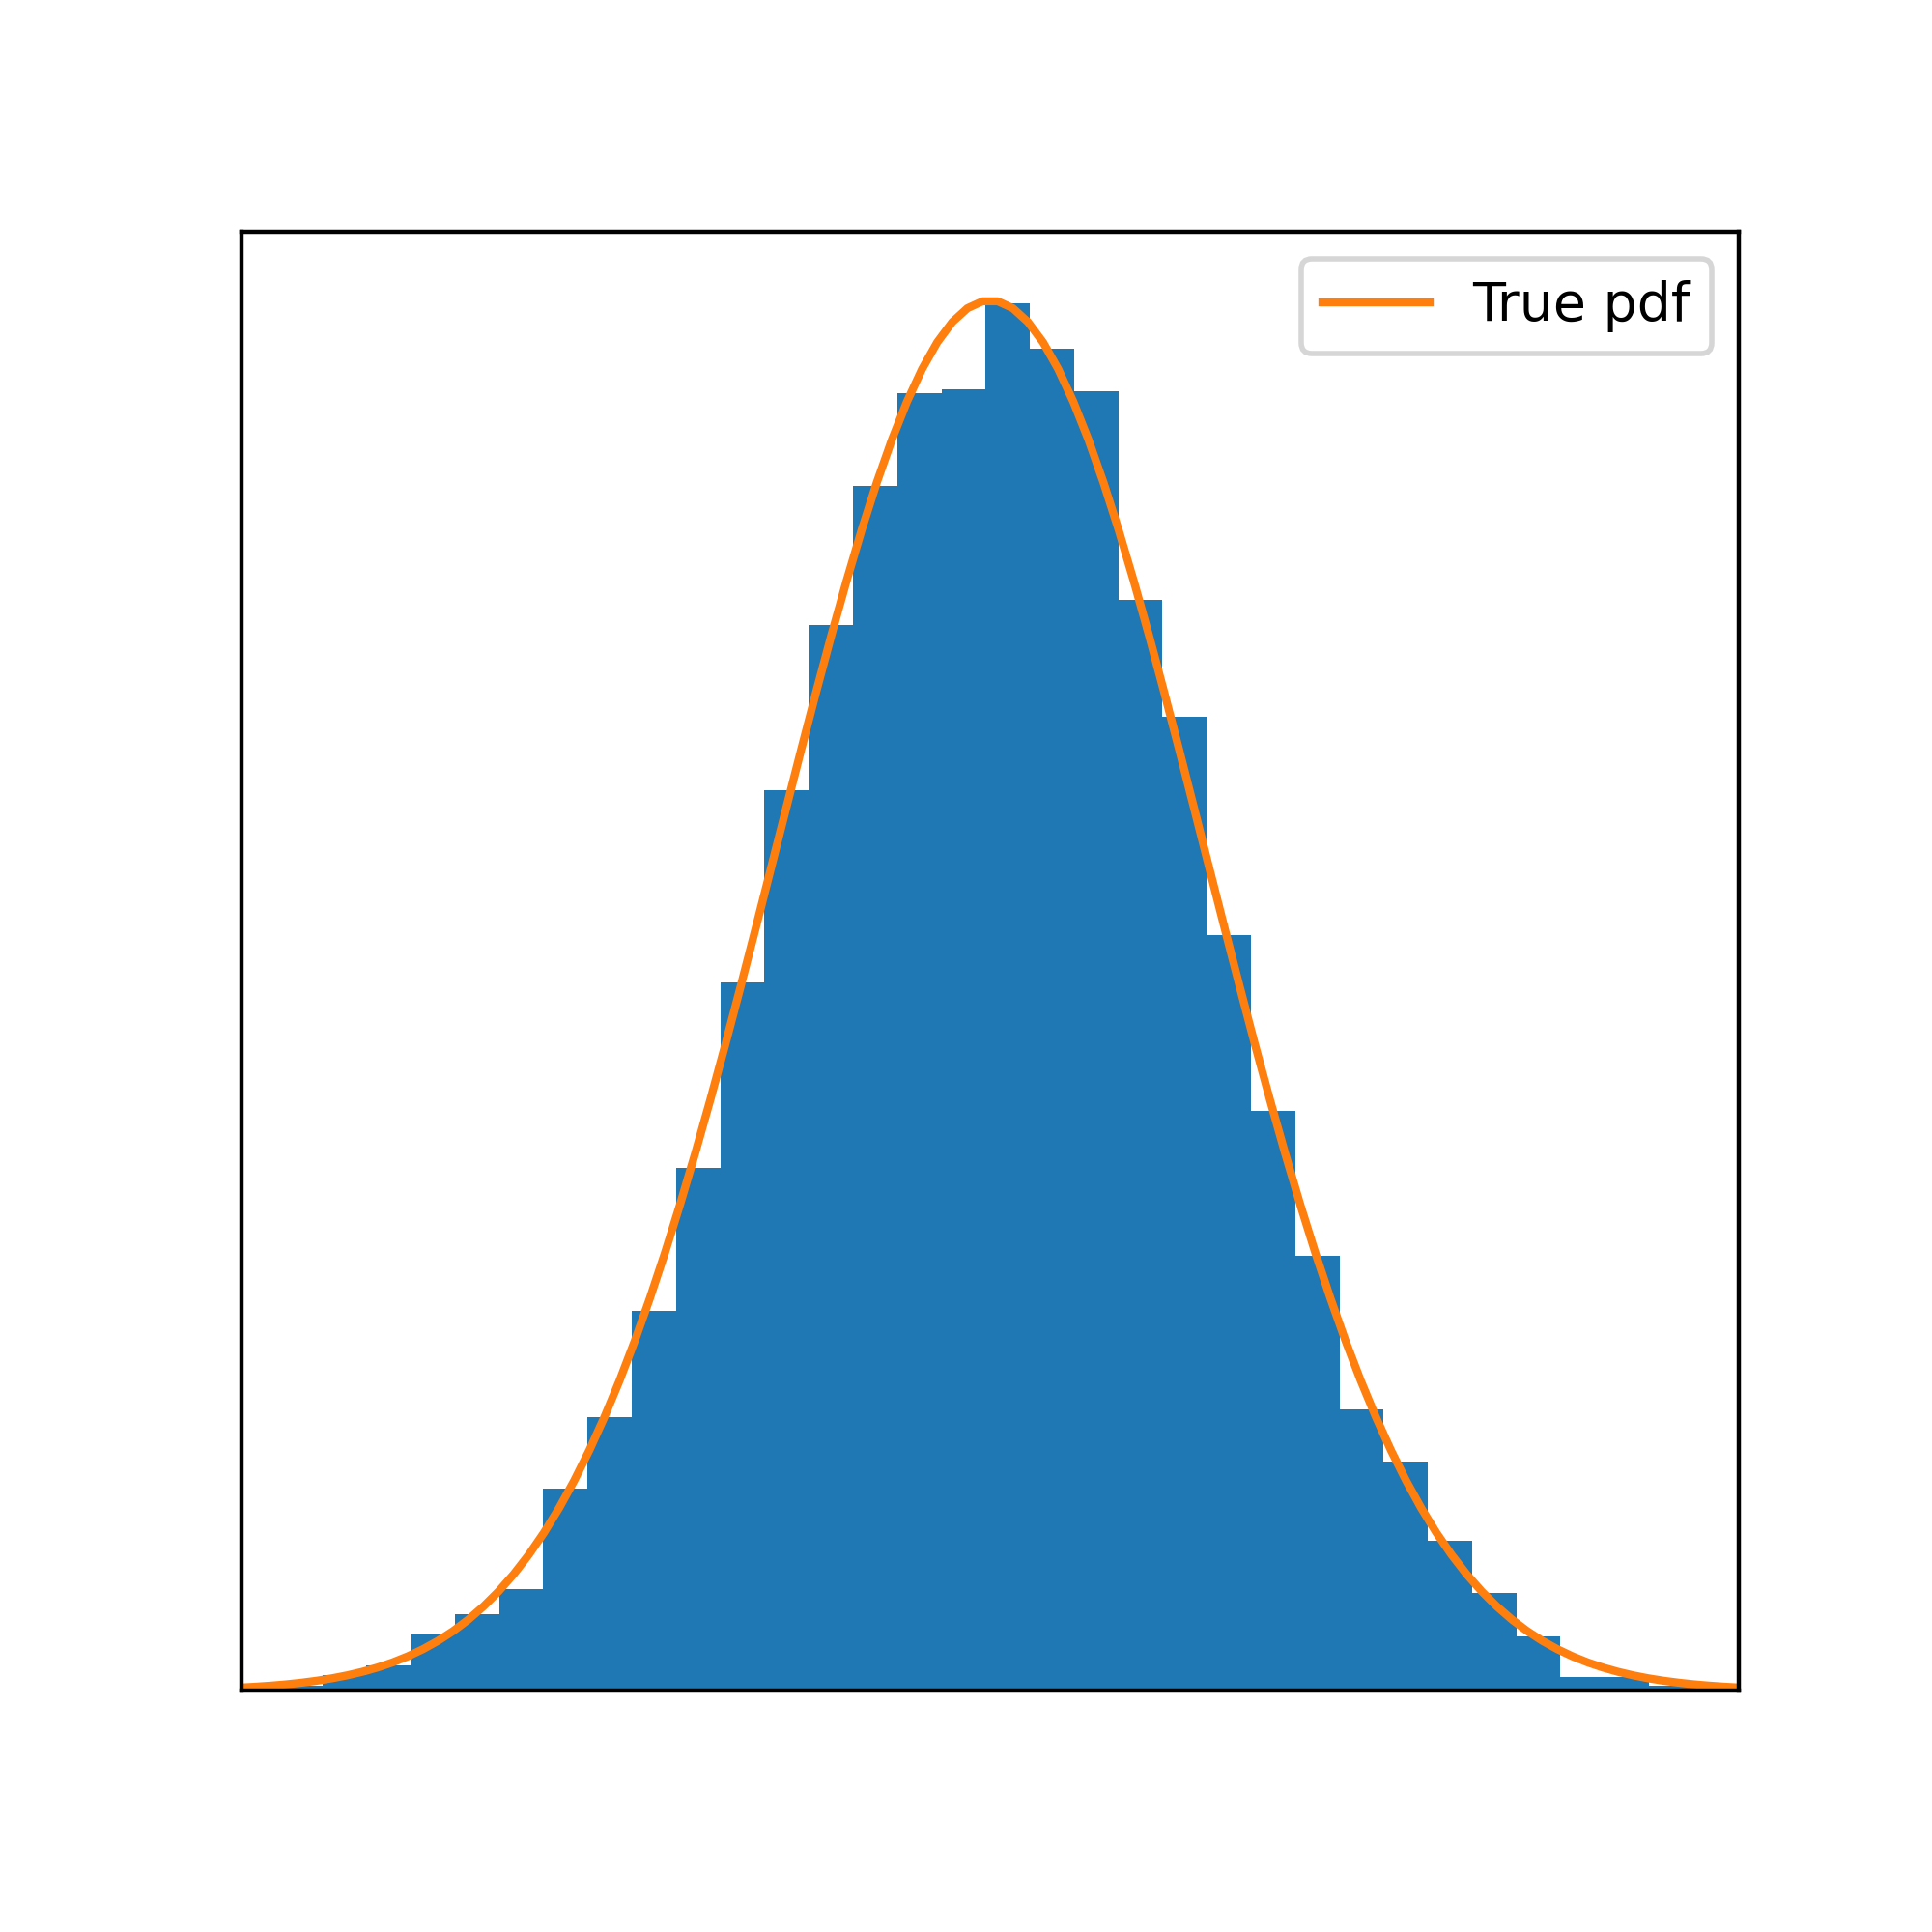
\includegraphics[width=1\linewidth]{img/gibbs/x2-hist.png}
      \caption{Empirical vs true marginal for $x_2$.}
    \end{subfigure}
    \centering
    \begin{subfigure}{.49\textwidth}
      \centering
      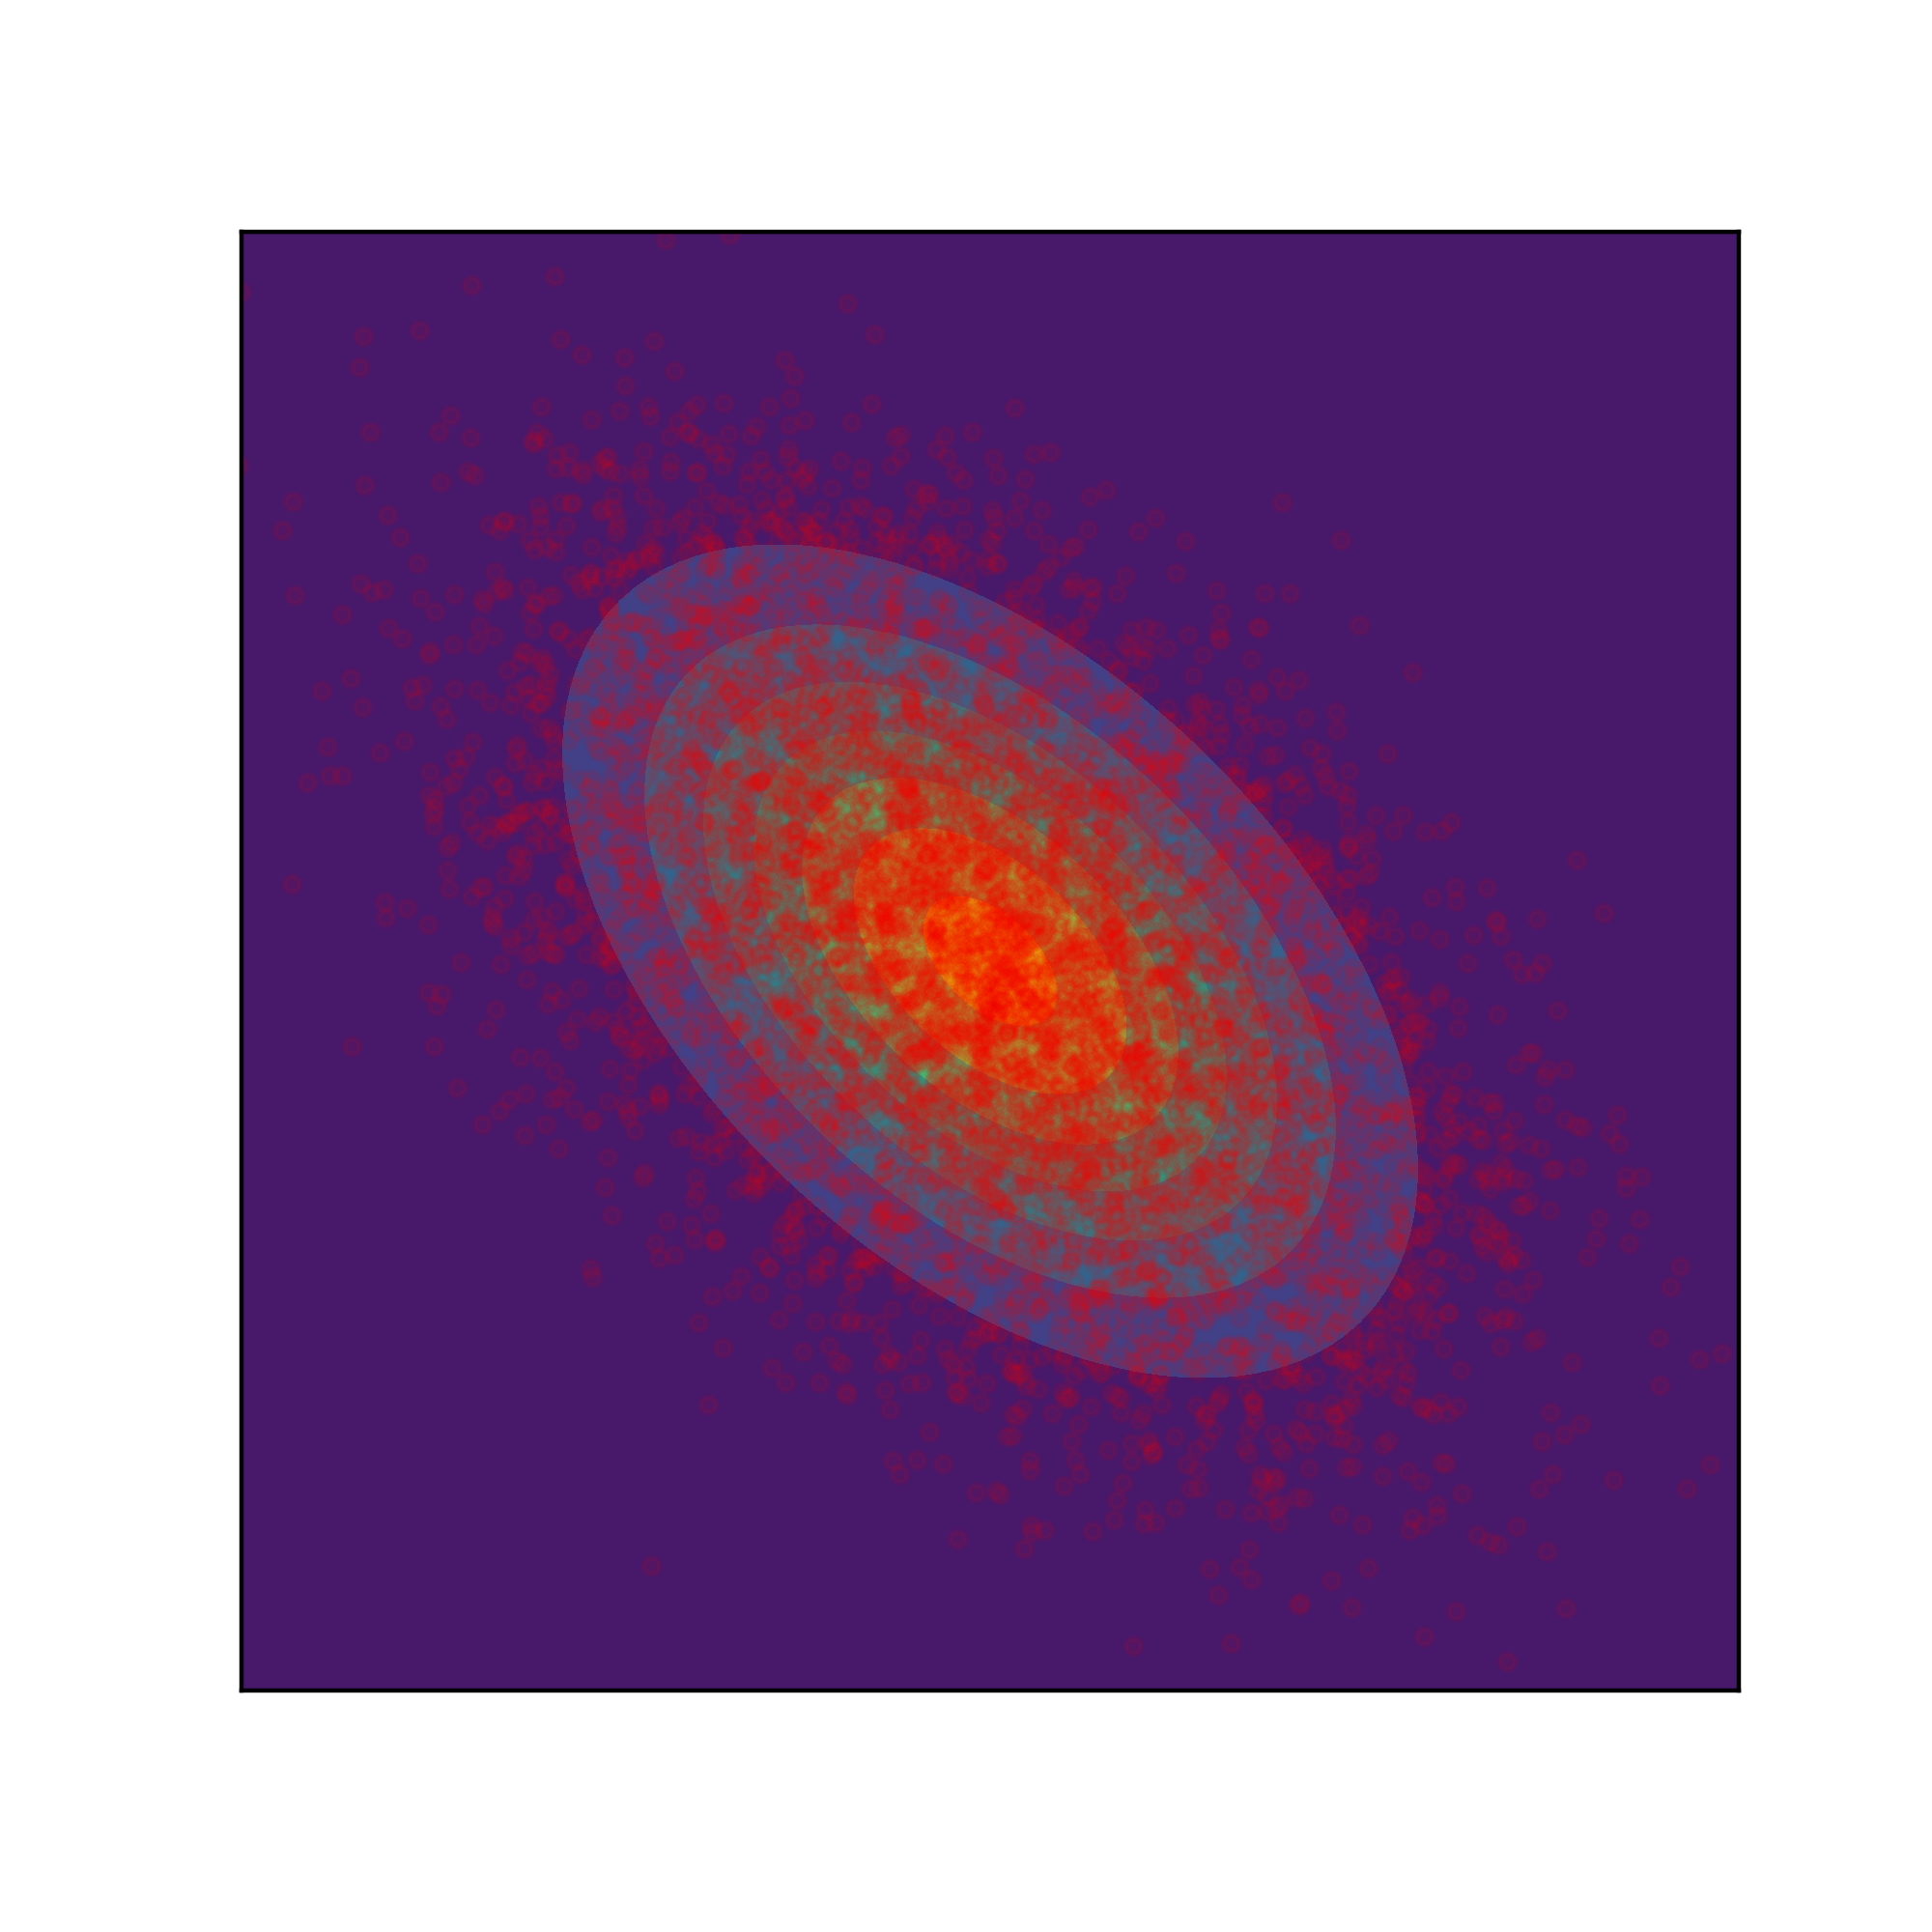
\includegraphics[width=1\textwidth]{img/gibbs/scatter.png}
      \caption{Empirical vs true marginal for $x_1, x_2$.}
    \end{subfigure}%
    \caption{Gibbs sampling a 2-D Gaussian.}
  \end{figure}


  \exercise
  \[
    p(x_1|x_2) = \mathcal{N}\left(x_1\left| \frac32 - \frac12 x_2, \frac34\right.\right)
  \]
  The formula for $p(x_2|x_1)$ is the same but with the indices switched.

  \exercise
  Given the structure of this model, we know that the posterior of $z_i$ is conditionally
  independent of $\mathbf{z}_{-i}$ given the cluster parameters. Thus, we can first sample $z_i$
  with
  \[
    p(z_i = k | x_i, \boldsymbol{\theta}) \propto
    \mathcal{N}(x_i| \mu_km, \sigma_k^2)\text{Cat}(z_i=k|\boldsymbol{\pi}).
  \]

  Next, we sample the cluster parameters using the semi-conjugate posterior
  $p(\mu_k, \sigma^2_k) = p(\mu_k)p(\sigma^2_k) = \mathcal{N}(\mu_k|m_0, v^2_0)
  \text{IG}(\sigma^2_k| a_0, b_0)$. It doesn't matter if we sample $\mu_k$ or $\sigma^2_k$ first.
  We sample $\mu_k$ from
  \[
    \mu_k \sim \mathcal{N}(m_{N_k}, v^2_{N_k})
  \]
  where $m_{N_k}, v^2_{N_k}$ is as defined in section 4.6.1, but only using the data points where
  $z_i=k$. Its the same process for $\sigma^2_k$, but with 
  \[
    \sigma^2_k \sim \text{IG}(a_{N_k}, b_{N_k})
  \]
  where $a_{N_k}$ and $b_{N_k}$ are given in section 4.6.2.2.

  \exercise
  I don't know any Matlab so I'm not going to try to modify the code. Gibbs sampling a Potts model
  is quite straightforward. Assuming that $w_{st} = J$ (see equation 19.22), we have
  \begin{equation}
    p(x_s=k| \mathbf{x}_{-s}) \propto e^{JN_{sk}}
  \end{equation}
  where $N_{sk}$ is the number of neighbours of $x_s$ with value $k$. To perform annealed sampling
  we first draw $k'$ from a proposed distribution (such as equation 1 or a uniform distribution),
  and then we set $\alpha$ to
  \[
    \alpha = \exp\left(\frac{JN_{sk} - JN_{sk'}}T\right)
  \]
  Where $k$ is the current value of $x_s$. We then set $x_s = k'$ with a probability of
  $\min(\alpha,1)$. We can rewrite the equation for $\alpha$ as 
   \[
     \alpha = \exp\left(\frac{J}T(N_{sk} - N_{sk'})\right).
  \]
  Thus we can see that increasing the temperature is equivalent to decreasing $J$, the coupling
  strength.

  \setcounter{exercise}{4}
  \exercise
  Recall that a Student distribution can be seen as an infinite mixture of Gaussians
  $\mathcal{N}(x|\mu, \sigma^2/z)$ where $z$ is unknown but follows a Gamma distribution 
  $\text{Ga}(\frac\upsilon2, \frac\upsilon2)$. We can first sample $z_i$ with equation 11.69 but
  using
  \[
    \delta_i = \left(\frac{y_i - \mathbf{w}^T \phi(\mathbf{x}_i)}{\sigma}\right)^2
  \]
  Now we have reduce the problem to weighted linear regression, here the weight for the $i$th data
  point is $1/z_i$. We can apply the results of section 7.6.1, but replacing $\sigma^{-2}$ with 
  $\sigma^{-2}\text{diag}(\mathbf{z})$.

  For $\sigma^2$, we can use the results of section 4.6.2.2, replacing equation 4.189 with
  \[
    b_N = b_0 + \frac12 \sum\limits_i^N (y_i - \mathbf{w}^T\phi(\mathbf{x}_i))^2 z_i.
  \]

  I was on the fence about doing this question, but it turned out to be pretty cool as the result
  used results from four chapters (4, 7, 11, and 24) and gave me a lot of confidence on my knowledge
  retention. Of course, I had to look up all the results from previous chapters, but at least I know
  where to look.

  \exercise
  Recall that Probit regression states that the difference in utilities between two options is
  Gaussian with $\sigma^2=1$ and $\mu_i = \mathbf{w}^T \mathbf{x}_i$. We can sample $z_i$ by drawing
  values $\mathcal{N}(\mathbf{w}^T \mathbf{x}_i, 1)$ until we draw a value with the same sign as
  $y_i$ (there are probably better ways of doing this, but I want to go to bed soon). Sampling
  $\mathbf{w}$ is just applying the results of 7.6.1, but replacing $y_i$ with $z_i$.
\end{document}
